\documentclass[10pt,twocolumn]{article}

% ---------------------------------------------------------------------------
% arxiv.sty is a single-column style: it renders the title in \scshape and
% builds the title block for \textwidth. Two overrides are needed for a
% two-column paper, and nothing else from the style is touched.
%
%   1. the class-level twocolumn option, with \twocolumn[{...}] supplying a
%      full-width title + abstract while the body flows in two columns;
%   2. a replacement \@maketitle, because \scshape would render the brand name
%      "DGUI-HyperMem" as small caps and destroy its casing, and because the
%      title block carries the project logo.
%
% Note: geometry and fancyhdr are deliberately NOT loaded -- arxiv.sty sets
% both and re-declaring them option-clashes.
% ---------------------------------------------------------------------------
\usepackage{arxiv}
\usepackage[T1]{fontenc}
\usepackage[utf8]{inputenc}
\usepackage{amsmath}
\usepackage{array}
% This MiKTeX resolves `nicefrac' to the SI-units helper, not the typography
% package booktabs expects, so \doublerulesep (read by booktabs at load time for
% \cmidrulesep) has to exist beforehand.
\providecommand{\doublerulesep}{2pt}
\usepackage{booktabs}
\usepackage{enumitem}
\usepackage{graphicx}
\usepackage{multirow}
\usepackage{microtype}
\usepackage{natbib}
\usepackage{url}
\usepackage{hyperref}
\usepackage{xcolor}
\usepackage{cleveref}
\usepackage{tikz}
\usetikzlibrary{decorations.pathmorphing,arrows.meta,calc}

\makeatletter
\renewcommand{\@maketitle}{%
  \begin{center}%
    % The mark sits above the title so the name and the product are one unit.
    \IfFileExists{figures/logo-dgui.png}{%
      \raisebox{-0.42cm}{
\includegraphics[height=1.5cm]{figures/logo-dgui.png}}%
      \\[0.30cm]%
    }{\mbox{}}%
    {\LARGE\bfseries \@title \par}%
    \vskip 0.62em
    {\rule{\textwidth}{0.4pt}}\\[0.42em]
    {\large \@author \par}%
    \vskip 0.16em
    {\normalsize \@affiliation \par}%
  \end{center}\par\vskip 1.1em}
\makeatother

% ---- hand-drawn (Excalidraw-style) figure kit ----------------------------
% Geometry is rectilinear; only the strokes wobble, which is what keeps the
% diagrams legible at 6-8pt in a two-column layout.
\tikzset{
  sk/.style={decorate,decoration={random steps,segment length=1.5pt,
        amplitude=.65pt},line width=.7pt,line cap=round,line join=round},
  skarrow/.style={sk,->,>={Stealth[length=3.2pt]}},
  kBox/.style={rounded corners=2.2pt,line width=.75pt,align=center,
        inner sep=2.6pt,font=\scriptsize,minimum height=7.4mm,fill opacity=.9},
  kInput/.style={kBox,draw=blue!62!black,fill=blue!11},
  kEmb/.style={kBox,draw=violet!62!black,fill=violet!13},
  kReason/.style={kBox,draw=green!50!black,fill=green!12},
  kLex/.style={kBox,draw=red!62!black,fill=red!11},
 kGate/.style={kBox,draw=orange!78!black,fill=orange!16},
  kQueue/.style={kBox,draw=red!70!black,fill=orange!20},
  kNeutral/.style={kBox,draw=black!62,fill=black!6},
  kTitle/.style={font=\footnotesize\bfseries},
}


\title{\texorpdfstring{DGUI-HyperMem: A Reasoning-Augmented Hybrid Memory\\
Service for LLM Agents on Serverless Infrastructure}{DGUI-HyperMem: A Reasoning-Augmented Hybrid Memory Service for LLM Agents on Serverless Infrastructure}}
\author{Wan Mohd Azizi bin Wan Hosen}
\makeatletter
\def\@affiliation{%
  CTECX Development \& Research\quad
  \IfFileExists{figures/logo-ctecx.png}{%
    \raisebox{-0.16cm}{
\includegraphics[height=0.62cm]{figures/logo-ctecx.png}}%
    \\[0.18em]%
  }{\mbox{}}%
  \texttt{dgui-hypermem.deckergui.my}}
\makeatother
\renewcommand{\shorttitle}{DGUI-HyperMem}
\renewcommand{\undertitle}{Technical Report}

\hypersetup{
  pdftitle={DGUI-HyperMem: A Reasoning-Augmented Hybrid Memory Service for LLM Agents on Serverless Infrastructure},
  pdfauthor={Wan Mohd Azizi bin Wan Hosen},
  pdfsubject={cs.AI; cs.CL; cs.SE},
  pdfkeywords={agent memory, retrieval augmentation, reciprocal rank fusion, MCP, serverless, Cloudflare Workers},
}

\begin{document}

\twocolumn[{\maketitle
\begin{abstract}
An agent that forgets is an agent that pays twice. This paper describes
DGUI-HyperMem (DeckerGUI HyperMemory), a long-term memory service for LLM agents
that runs entirely on a serverless edge runtime, is addressed over the Model
Context Protocol, and is designed so that an agent's memory is queried
\emph{by the agent itself} rather than replayed as prompt text. The system fuses
approximate-nearest-neighbour search over a 768-dimensional vector index with
BM25 over an external-content FTS5 index by reciprocal rank fusion, then submits
the fused shortlist to a reasoning layer that re-ranks and re-scores it. A
write path assigns every memory a type, a salience and a durability judgement,
suppresses low-signal content behind a calibrated salience gate, and
automatically supersedes memories that a newer write contradicts. We contribute
a description of the architecture and its exact scoring and gating constants; a
privacy argument for why redaction must happen at enqueue rather than at export,
motivated by an incident in which a passkey reached a public dataset; and a
simulated retrieval evaluation built on the production embedding model. That
evaluation returns a negative result about the deployed configuration:
equal-weight rank fusion is \emph{worse} than the dense channel alone
($0.378$ against $0.418$ nDCG@10), because reciprocal rank fusion discards score
magnitudes and so lets a weak lexical channel dilute a strong dense one.
Re-weighting the lexical channel to $0.3$ recovers the loss and edges past the
best single channel ($0.422$, with recall@10 rising from $0.598$ to $0.624$),
which localises the defect to the weights rather than to the fusion. We also
find that the judgement stage is not a precision win but a recall and
difficulty trade, and we report it as such. The evaluation is explicitly a
simulation of long-horizon engineering-agent memory and is not a DeepSWE result;
we state the distinction and the threats to validity it carries. The reasoning
corpus exported by the service is public, which makes the curation pipeline
itself reproducible.
\end{abstract}
\vspace{0.55em}
\keywords{agent memory \and reciprocal rank fusion \and Model Context Protocol
\and serverless retrieval \and knowledge curation}
}]

% ===========================================================================
\section{Introduction}
\label{sec:intro}

Retrieval-augmented generation established that grounding a model in external
text beats memorising it. Agent memory asks the same question about the agent
itself. Across a long session, and across sessions, an agent accumulates facts,
decisions, stated preferences, and hard-won diagnoses; on the next task those
observations are usually not in the context window, and if they are not
retrieved they are simply lost. The cost is not only accuracy. Re-deriving a
decision the agent already made wastes tool calls, and re-discovering a
diagnosed failure is the most expensive kind of mistake an autonomous agent
makes, because the symptom has usually already been paid for once.

The mechanical solution is a vector store with a similarity search. It is a good
solution to the wrong question. Real engineering memory is not uniformly
semantic. A developer asking ``where is the migration runner'' wants a path
match, and no embedding model is reliably better at that than a token match.
A developer asking ``why did we pick Kafka here'' wants a rationale, and the
rationale rarely shares content words with the question. A single dense index
handles the second case badly and the first adequately; a single lexical index
does the reverse. The interesting engineering is in what happens between the two
channels and after them.

DGUI-HyperMem is a deployed memory service that takes this seriously. It is a
single Cloudflare Worker binding SQLite (D1), a vector index (Vectorize), and a
model runtime (Workers AI), exposed to any MCP-capable client\citep{anthropic2025mcp}
at one URL. Its central claim is that a memory service should not merely
\emph{retrieve} but should \emph{judge}: a reasoning layer inspects the fused
shortlist and decides which candidate actually answers the question. Every
decision that reasoning layer makes is recorded, redacted, and exported as
training data, so the judgement improves rather than being rewritten each
deployment.

\subsection{Contributions}

\begin{enumerate}[leftmargin=1.15em,itemsep=1pt,topsep=2pt]
\item An architecture and an exact transcription of the deployed retrieval and
      curation constants --- reciprocal rank fusion at $K=60$, the salience gate
      at $3.0$, the supersede threshold at $0.80$, and the two linear scoring
      blends --- so that the system is reproducible rather than merely
      described (\cref{sec:read,sec:write}).
\item A privacy argument for redaction at enqueue. Redacting at export is too
      late, and we show why with an incident in which a real credential was
      written to a public dataset by a pipeline whose only redaction pass ran
      afterwards (\cref{sec:privacy}).
\item A simulated retrieval evaluation over a synthetic long-horizon workload,
      using the same embedding model as the deployed index, that varies the
      fusion weights and the re-ranking stage independently and reports where
      each one loses accuracy rather than where it gains it (\cref{sec:eval}).
\item A positioning against other agent-memory systems along axes that matter
      operationally rather than aspirationally (\cref{sec:related}).
\end{enumerate}

We make no claim to beat a purpose-built memory service on a shared benchmark.
We make a narrower claim, which is that the design decisions described here are
coherent, that their constants are calibrated against observed behaviour, and
that the component that matters most --- a judgement stage over the fused
shortlist --- is the one most often omitted from comparable systems.

% ===========================================================================
\section{Background}
\label{sec:background}

\subsection{Two retrieval channels and their failure modes}

Let $D$ be a memory store, $q$ a query, and $d$ a memory. A lexical ranker
scores
\begin{equation}
\mathrm{BM25}(q,d)=\sum_{t\in q}\mathrm{idf}(t)\,
  \frac{tf(t,d)\,(k_1{+}1)}{tf(t,d)+k_1\!\left(1-b+b\frac{|d|}{\bar{|d|}}\right)},
  \label{eq:bm25}
\end{equation}
with $k_1=1.2$ and $b=0.75$. Its strength is exact-match on rare tokens: file
paths, identifiers, error strings. Its weakness is that it needs the query and
the memory to share a token, so a paraphrase is invisible to it. A dense ranker
scores $q^\top d / (\lVert q\rVert \lVert d\rVert)$ over an embedding, and
behaves in the mirror-image way. Our evaluation quantifies the mirror image
directly: over paraphrase queries whose gold memory shares no content word with
the question, lexical retrieval scores $0.164$ nDCG@10 while dense retrieval
scores $0.713$ (\cref{sec:eval}). That gap is the entire motivation for running
two channels, and \cref{sec:eval} also shows that naively fusing them destroys
most of it.

Reciprocal rank fusion \citep{cormack2009rrf} combines ranked lists without
requiring comparable scores, which is exactly the situation here: BM25
magnitudes are corpus-dependent and cosine magnitudes are model-dependent, so
any linear blend of the two raw scores would need per-corpus calibration.
RRF instead consumes rank positions:
\begin{equation}
\mathrm{RRF}(d)=\sum_{\ell\in\mathcal{L}}\frac{1}{K+\mathrm{rank}_{\ell}(d)},
\label{eq:rrf}
\end{equation}
over rank lists $\mathcal{L}$, with $K=60$. The constant damps the head of each
list, which prevents a single channel's top hit from dominating purely by being
first.

\subsection{Agent memory systems}
\label{sec:related}

Several mature systems store memory for agents. We compare them along the
axes that determine whether a service can be run and trusted, and defer the
full table to \cref{tab:compare}.

\emph{mem0} offers an extract-and-store pipeline over a vector store with
optional BM25 and entity boosting, and reports strong long-conversation
benchmarks \citep{chhikara2025mem0}. Its April 2026 algorithm revision is
explicitly single-pass: memories accumulate and nothing is overwritten, which
is a deliberate choice against the cost of an agentic loop at write time. Its
read path fuses several signals but does not spend a model call on
re-ranking.

\emph{Zep} \citep{zep2025} maintains a temporal knowledge graph and exposes it
through a managed cloud service, with Graphiti as the open-source engine.
Temporal structure is a real advantage for questions about state and ordering;
it also imposes a graph-extraction step and an entity-resolution problem that a
row-and-vector store does not have.

\emph{Letta} \citep{letta2025} treats memory as an agent feature rather than a
service: the agent is the stateful object, and memory blocks are part of its
context construction. This is a different integration contract from a memory
endpoint another tool can call.

\emph{Cognee} and the reference \emph{MCP knowledge-graph memory server}
\citep{mcpserver2025} bracket the design space at the other end. The latter is
deliberately minimal --- entities, relations, observations, held in a local JSON
file --- which makes it an excellent teaching artifact and a poor production
service.

The gap we occupy is specific: a memory service that is (i) reachable over MCP,
(ii) self-hostable on infrastructure the operator already pays for, (iii) hybrid
rather than purely dense, (iv) willing to spend a reasoning call to reorder a
shortlist, and (v) transparent about the training data its own reasoning
generates.

% ===========================================================================
\section{System Overview}
\label{sec:system}

\Cref{fig:arch} shows the deployed topology. A Cloudflare Worker is the entire
service: there is no container, no orchestrator, and no separate inference
service. Three bindings carry the state.

\begin{figure*}[t]
\centering
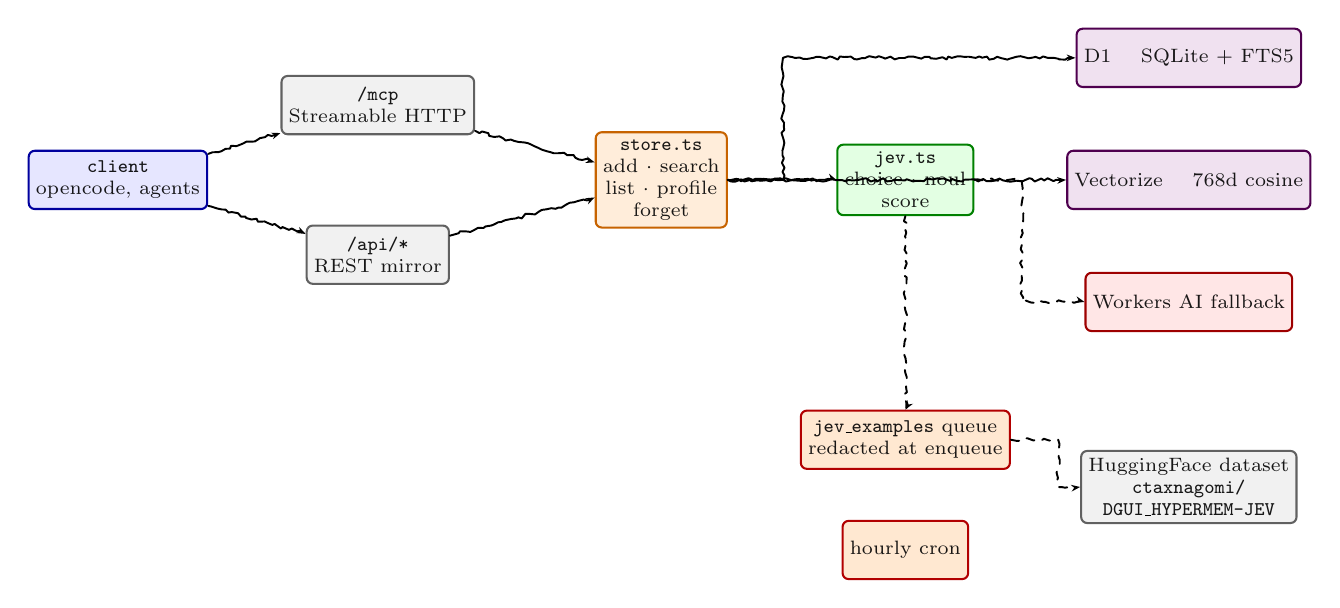
\begin{tikzpicture}[x=1cm,y=1cm]
\node[kInput]   (cli)  at (1.2,0)     {\texttt{client}\\opencode, agents};
\node[kNeutral]   (mcp)  at (4.5,0.95)  {\texttt{/mcp}\\Streamable~HTTP};
\node[kNeutral]   (api)  at (4.5,-0.95) {\texttt{/api/*}\\REST mirror};
\node[kGate] (store)at (8.1,0)     {\texttt{store.ts}\\add $\cdot$ search\\list $\cdot$ profile\\forget};
\node[kReason]  (jev)  at (11.2,0)    {\texttt{jev.ts}\\choice $\cdot$ noul\\score};
\node[kEmb] (d1)   at (14.8,1.55) {D1 \quad SQLite + FTS5};
\node[kEmb] (vec)  at (14.8,0)    {Vectorize \quad 768d cosine};
\node[kLex]    (ai)   at (14.8,-1.55){Workers AI fallback};
\node[kQueue]  (q)    at (11.2,-3.3) {\texttt{jev\_examples} queue\\redacted at enqueue};
\node[kQueue]  (cron) at (11.2,-4.7) {hourly cron};
\node[kNeutral]   (hf)   at (14.8,-3.9) {HuggingFace dataset\\\texttt{ctaxnagomi/}\\\texttt{DGUI\_HYPERMEM-JEV}};

\draw[skarrow] (cli) -- (mcp);
\draw[skarrow] (cli) -- (api);
\draw[skarrow] (mcp) -- (store);
\draw[skarrow] (api) -- (store);
\draw[skarrow] (store) -- (jev);
\draw[skarrow] (store.east) -- ++(0.7,0) |- (d1.west);
\draw[skarrow] (store.east) -- ++(0.7,0) |- (vec.west);
\draw[skarrow,dashed] (jev.east) -- ++(0.6,0) |- (ai.west);
\draw[skarrow,dashed] (jev.south) -- (q.north);
\draw[skarrow,dashed] (q.east) -- ++(0.6,0) |- (hf.west);
\end{tikzpicture}
\caption{Deployed topology. Solid arrows are request paths; dashed arrows are
write-side analysis and asynchronous dataset export. The two protocols are
equivalent surfaces over one implementation, so a non-MCP client loses nothing
but the tool schema.}
\label{fig:arch}
\end{figure*}

\begin{description}[leftmargin=0pt,itemsep=1pt,topsep=2pt,parsep=0pt]
\item[D1 (SQLite).] Rows of memory, plus an external-content FTS5 table kept in
      sync by insert, update, and delete triggers, so the lexical index cannot
      drift from its source of truth. \texttt{porter unicode61} stemming makes
      the lexical channel insensitive to inflection.
\citep{cloudflare2025d1}
\item[Vectorize.] 768-dimensional vectors, cosine metric, filtered by scope and
      status at query time so that superseded rows leave both channels at once.
\citep{cloudflare2025vectorize}
\item[Workers AI.] The reasoning backend, used both as the primary judge and as
      the fallback when the primary is unavailable.\citep{cloudflare2025workers}
\end{description}

The service exposes nine tools (\cref{tab:tools}). The set is deliberately small
because an agent's tool budget is finite and a memory service competes with the
agent's actual work for that budget.

\begin{table}[t]
\caption{The MCP tool surface. Destructive tools are annotated as such so an
agent can gate on it; \texttt{sync\_jev\_dataset} is the only tool with an
effect outside the caller's own scope.}
\label{tab:tools}
\centering\footnotesize
\begin{tabular}{@{}lp{0.52\columnwidth}@{}}
\toprule
Tool & Purpose \\
\midrule
\texttt{add}      & Store a memory; assigns type and salience, supersedes contradicted rows \\
\texttt{search}   & Hybrid recall then re-rank; returns scored memories \\
\texttt{suggest}  & Detect repeats, find related rows, propose generation \\
\texttt{list}     & Browse a scope, newest first \\
\texttt{profile}  & Totals, counts by type, top tags, mean salience \\
\texttt{forget}   & Delete by id, by query, or a whole scope (destructive) \\
\texttt{help}     & Describe the server and its tools \\
\texttt{sync\_jev\_dataset} & Flush queued decision rows to the public dataset \\
\texttt{jev\_queue\_stats}  & Pending, uploaded, and failed counts by use case \\
\bottomrule
\end{tabular}
\end{table}

% ===========================================================================
\section{Write Path}
\label{sec:write}

\Cref{fig:write} is the write path. Four things happen, in this order, and the
order is the design.

\begin{figure}[t]
\centering
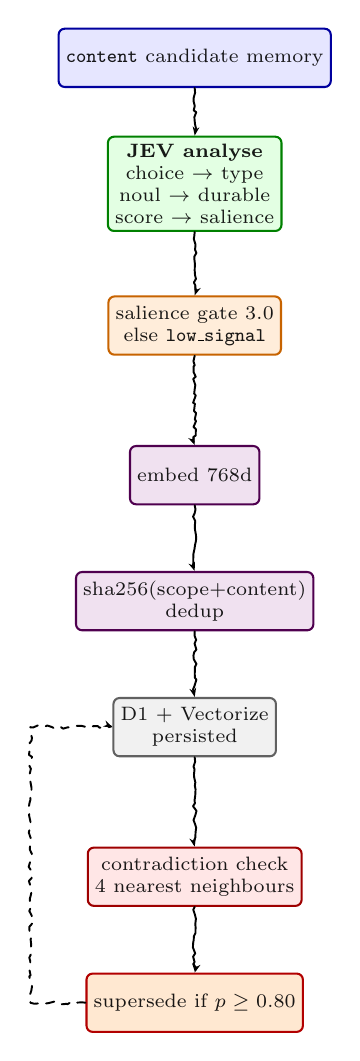
\begin{tikzpicture}[x=1cm,y=1cm]
\node[kInput]   (in)    at (2.1,4.5) {\texttt{content} candidate memory};
\node[kReason]  (an)    at (2.1,2.9) {\textbf{JEV analyse}\\choice $\to$ type\\noul $\to$ durable\\score $\to$ salience};
\node[kGate] (gate)  at (2.1,1.1) {salience gate $3.0$\\else \texttt{low\_signal}};
\node[kEmb] (emb)   at (2.1,-0.8) {embed $768$d};
\node[kEmb] (ded)   at (2.1,-2.4) {sha256(scope+content)\\dedup};
\node[kNeutral]   (st)    at (2.1,-4.0) {D1 + Vectorize\\persisted};
\node[kLex]    (chk)   at (2.1,-5.9) {contradiction check\\4 nearest neighbours};
\node[kQueue]  (sup)   at (2.1,-7.5) {supersede if $p\geq0.80$};
\draw[skarrow] (in)--(an);
\draw[skarrow] (an)--(gate);
\draw[skarrow] (gate)--(emb);
\draw[skarrow] (emb)--(ded);
\draw[skarrow] (ded)--(st);
\draw[skarrow] (st)--(chk);
\draw[skarrow] (chk)--(sup);
\draw[skarrow,dashed] (sup.west) -- ++(-0.7,0) |- (st.west);
\end{tikzpicture}
\caption{Write path. The reasoning call precedes persistence, so a memory is
never stored without its judgements; the contradiction check follows
persistence, so it can compare against what is already there.}
\label{fig:write}
\end{figure}

\paragraph{Refusal before analysis.}
Content matching a prohibited pattern --- live Stripe or GitHub credentials,
AWS keys, PEM private keys, exploit references, or child sexual abuse material
--- is rejected before any model is called and before anything is stored. This
is a hard refusal, not a redaction: the content is never written, so it cannot
reach the dataset pipeline.

\paragraph{One reasoning pass, three judgements.}
\Cref{sec:jev} describes the layer. For the write path it yields a type, a
duribility score, and a salience score.

\paragraph{The salience gate.}
Salience is an ordinal score on a five-point scale, so the natural question is
where to cut. The deployed default is $3.0$, and the comment in the source is
worth repeating because it records a calibration failure: a threshold of $4.0$
``filtered everything in this dataset'', while $3.0$ sits at the model's median.
A gate set from intuition rather than from the observed score distribution is
the single most common way a curation layer becomes a memory \emph{deleter},
because it does not fail loudly --- it simply never stores anything.

\paragraph{Deduplication by content hash.}
The hash is taken over scope and normalised content, with a unique index on the
pair. A repeated add updates the existing row rather than creating a second one.

\paragraph{Contradiction and supersession.}
After persisting, the system queries the four nearest neighbours and asks the
reasoning layer for the probability that the incoming memory contradicts each.
Above $p\geq0.80$ the earlier row is marked superseded, its vector is deleted,
and the supersession is logged. Rows are never destroyed, so a superseded
memory is still recallable by id, which is what makes \cref{sec:eval}'s temporal
queries answerable at all.

% ===========================================================================
\section{Read Path}
\label{sec:read}

\Cref{fig:recall} is the read path: two channels, a fusion, a judgement, and a
blend.

\begin{figure*}[t]
\centering
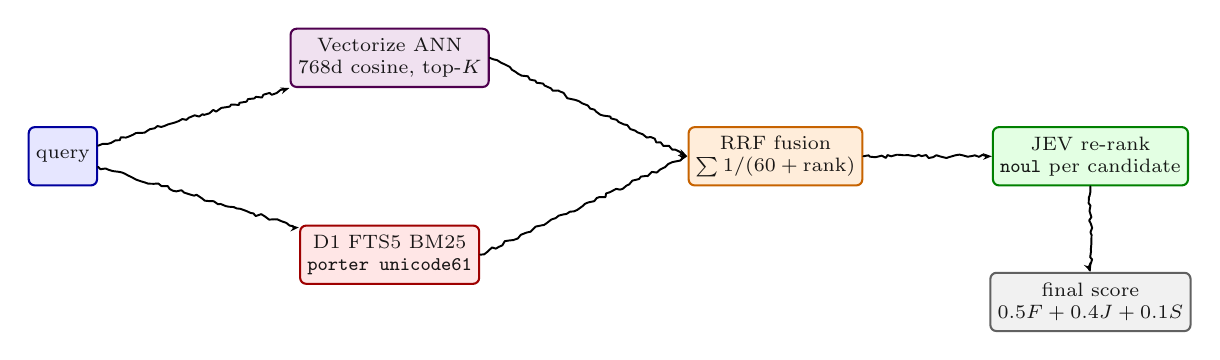
\begin{tikzpicture}[x=1cm,y=1cm]
\node[kInput]   (q)  at (0.85,0)     {query};
\node[kEmb] (v)  at (5.0,1.25)  {Vectorize ANN\\$768$d cosine, top-$K$};
\node[kLex]    (k)  at (5.0,-1.25) {D1 FTS5 BM25\\\texttt{porter unicode61}};
\node[kGate] (f)  at (9.9,0)      {RRF fusion\\$\sum 1/(60+\mathrm{rank})$};
\node[kReason]  (j)  at (13.9,0)     {JEV re-rank\\\texttt{noul} per candidate};
\node[kNeutral]   (s)  at (13.9,-1.85) {final score\\$0.5F+0.4J+0.1S$};
\draw[skarrow] (q) -- (v);
\draw[skarrow] (q) -- (k);
\draw[skarrow] (v.east) -- (f.west);
\draw[skarrow] (k.east) -- (f.west);
\draw[skarrow] (f) -- (j);
\draw[skarrow] (j) -- (s);
\end{tikzpicture}
\caption{Hybrid recall. The shortlist handed to the reasoning layer is bounded
($\max(2k,12)$ candidates at the deployed settings), so the cost of judging is
capped independently of store size.}
\label{fig:recall}
\end{figure*}

\paragraph{Two channels, filtered identically.}
Both channels are scoped and filtered to \texttt{status = 'active'}, so a
superseded row is invisible to both. Filtering only one channel would let a
retired memory re-enter through the other, which is precisely the staleness
failure the supersede logic exists to prevent.

The lexical channel builds an FTS5 \texttt{MATCH} query from up to sixteen
stemmed tokens joined by \texttt{OR}. The dense channel issues a filtered
vector query with the same limit.

\paragraph{Fusion.}
\Cref{eq:rrf} with $K=60$ over the two rank lists. The fused score is
normalised by the maximum fused score in the candidate set, giving
$F\in[0,1]$, and the top $\max(2k,12)$ candidates form the shortlist.

\paragraph{Judgement.}
The reasoning layer scores every shortlisted candidate for relevance on the same
bounded scale the write path uses. This is the one step that costs a model call,
and it is bounded by the shortlist rather than by the store.

\paragraph{The blend.}
Let $S=\mathrm{clamp}((\mathrm{salience}\text{ or }2)/4,0,1)$ be the normalised
salience and $J$ the bounded relevance judgement. When a judgement is available
the final score is
\begin{equation}
\mathrm{score}(d)=0.50\,F(d)+0.40\,J(d)+0.10\,S(d),
\label{eq:blend}
\end{equation}
and when the reasoning backend is unavailable the judgement term is dropped and
its weight given to fusion,
\begin{equation}
\mathrm{score}(d)=0.85\,F(d)+0.15\,S(d).
\label{eq:blendfallback}
\end{equation}
The weighting is a considered trade rather than a tuned constant. Fusion is the
component with the most evidence behind it, so it carries half the weight even
when a judgement is available, and the overwhelming majority when one is not.
Salience is retained in both cases at a small weight, because a memory the model
considered important is weak evidence that a user who asked about it wanted it.
Every term is in $[0,1]$: this is a design constraint on the reasoning backend,
not an afterthought, and \cref{sec:eval} shows that feeding an unbounded score
into the $0.40$ slot distorts the blend.

Results are sorted by \cref{eq:blend} and truncated to $k$. Returned rows have
their access counters touched and the search is logged with candidate and
result counts, which is what makes the profile tool and the queue statistics
possible without a second telemetry path.

% ===========================================================================
\section{The JEV Reasoning Layer}
\label{sec:jev}

The layer exposes three primitives and nothing else \cref{fig:jev}. The
restriction is deliberate: a small, fixed verb set makes the recorded training
rows comparable to live inputs, because the instruction block is the same object
in both.

\begin{figure}[t]
\centering
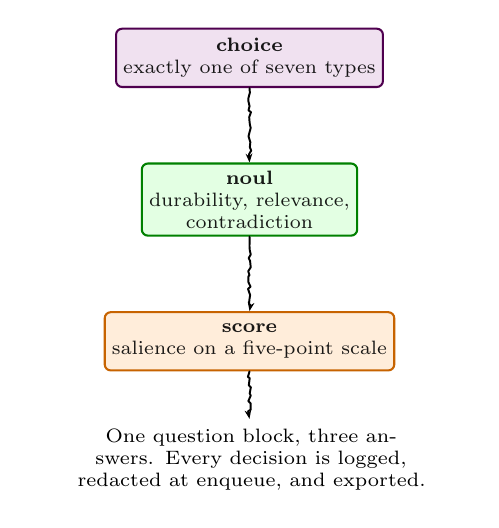
\begin{tikzpicture}[x=1cm,y=1cm]
\node[kEmb] (c) at (2.6,1.5) {\textbf{choice}\\exactly one of seven types};
\node[kReason]  (n) at (2.6,-0.3) {\textbf{noul}\\durability, relevance,\\contradiction};
\node[kGate] (s) at (2.6,-2.1) {\textbf{score}\\salience on a five-point scale};
\node[font=\scriptsize,align=center,text width=5.4cm] (note) at (2.6,-3.6)
  {One question block, three answers. Every decision is logged, redacted at enqueue, and exported.};
\draw[skarrow] (c)--(n);
\draw[skarrow] (n)--(s);
\draw[skarrow] (s.south)--(note.north);
\end{tikzpicture}
\caption{The reasoning primitives. \texttt{choice} runs once per memory;
\texttt{noul} runs per write, per shortlisted candidate, and per contradiction
test; \texttt{score} runs per write.}
\label{fig:jev}
\end{figure}

\paragraph{Seven types.}
Fact, preference, decision, project, solution, architecture, and conversation.
The \emph{conversation} type exists so that session-only chatter has somewhere
to go; a memory store with no such category either keeps trivia forever or
throws it away, and both failure modes are worse than labelling it.

\paragraph{Three backends.}
The layer resolves to a hosted reasoning backend, a Workers AI emulation of the
same three primitives, or off. The \emph{off} path is a real mode, not an
error: it makes \cref{eq:blend}'s first branch the normal operation, which is
why that branch exists and why it is specified rather than left as undefined
behaviour.

\paragraph{Bounded outputs.}
Every primitive returns a value in $[0,1]$. The scoring blend depends on this
contract. It is a genuine coupling, not a formality, and it is the kind of
detail that is usually left implicit and then violated by the first backend
added.

% ===========================================================================
\section{Privacy: Redact at Enqueue}
\label{sec:privacy}

The reasoning corpus this service exports is public, by design: it is the
training set for the reasoning layer, and a curation corpus nobody can inspect
is not a research contribution. That makes the export path a disclosure surface,
and it constrains where redaction must happen.

\paragraph{The failure we are arguing about.}
An earlier revision of this system redacted \emph{at export}. The queue held
rows verbatim; the sync job read them, redacted, and uploaded. A real
administrator passkey was stored as memory during ordinary use, the row was
queued, and the redaction pass did not match it. The credential was published.
The dataset was corrected, but the value had been public, and a rotating
credential does not undo a publish.

The generalisation is the argument: redaction at export is a promise about a
code path that runs on someone else's data, in a batch job, at an hour nobody
is watching. Redaction at enqueue is a property of the write path, exercised on
every row, in the same request that stores it.

\paragraph{How the enqueue pass works.}
Two layers. Unambiguous provider formats are matched directly: OpenAI
\texttt{sk-}, Stripe \texttt{sk\_live\_} and \texttt{whsec\_}, GitHub
\texttt{ghp\_} and \texttt{github\_pat\_}, HuggingFace \texttt{hf\_},
Cloudflare \texttt{cfat\_}, Slack \texttt{xox}, AWS \texttt{AKIA}, Google
\texttt{AIza}, and JWTs.

The interesting case is the ambiguous one. A generic
\emph{credential-assignment} rule requires a credential keyword
(\texttt{passkey}, \texttt{api\_key}, \texttt{bearer\_token}, ...) followed by a
delimiter or a bounded copula chain, then a value. Three details make it usable
rather than destructive. The separator permits at most four stacked words,
which lets it reach ``rotating the passkey \emph{to new value} \texttt{x}'' while
preventing the rule from chaining across a sentence. A plausibility gate rejects
values that cannot be secrets: anything under six characters, bare digits, and
anything on a denylist of ordinary technical vocabulary, so that ``wrapped in
\texttt{base64}'' and ``the token authentication'' survive intact. And the rule
reports \emph{which} rule fired, never the value, so a log line is safe to
publish.

\paragraph{Identity fields are whitelisted, not blacklisted.}
Row metadata needed for slicing the dataset --- use case, instruction type,
provider, model, timestamps --- is passed through untouched, and everything else
is walked recursively, because free text appears both as top-level JSON strings
and nested inside \texttt{state}, \texttt{questions}, and \texttt{answers}. A
blacklist of known-sensitive keys would have missed the nested copies; walking
non-identity fields does not.

\paragraph{What this does not do.}
We state plainly: pattern matching is not entropy analysis. A secret in an
unfamiliar format, or one with no credential keyword near it, will pass. This
layer raises the cost of an accident; it does not make disclosure safe. The
conclusion is architectural --- treat any exported corpus as public, and design
the pipeline so that being wrong is survivable --- rather than a claim that the
rules are complete.

% ===========================================================================
\section{Evaluation}
\label{sec:eval}

\subsection{What this evaluation is, and is not}

DeepSWE~\citep{deepswe} is a real software-engineering agent benchmark.
Running it requires paid proprietary endpoints and an air-gapped runner. Neither is available to us, and a fabricated score attributed to it
would be worse than no score. This section therefore reports a
\emph{simulation} of the memory behaviour such a benchmark exercises:
persistent facts, stated rationales, symptom-and-fix records, configuration
that evolves across sessions, and contradictions between them. We make no claim
about DeepSWE performance and our harness is not derived from it.

\subsection{Harness}

A seeded generator builds a synthetic engineering repository and a memory store
of roughly $870$ rows across $95$ sessions. Twenty subjects are given supersede
chains of length two to four, so that answering ``what does this use \emph{now}''
requires the whole chain to have been maintained rather than one stale row
filtered. The remainder is filler chosen to be realistic distractors: decisions,
diagnoses, conventions, and low-value chatter that a good system should rank
last.

Every query is planted alongside the memory that answers it, so relevance is
never model-judged. Queries fall into four classes: \emph{lexical}, which
requires an exact rare token such as a path; \emph{semantic}, which is a
paraphrase sharing no content word with its gold memory; \emph{temporal}, which
asks for the current state of an evolving subject or for an earlier generation;
and \emph{pinpoint}, which asks for a rationale or a diagnosis. Each class is
generated to a quota before truncation, so that limiting the query count does not
silently drop the smallest class: the reported mix is $37$ lexical, $39$
pinpoint, $37$ semantic and $37$ temporal per seed, $150$ in total, over three
seeds.

\subsection{What is faithful and what is substituted}

Being explicit here matters more than any single number. The dense channel uses
\texttt{BAAI/bge-base-en-v1.5}\citep{ding2021bge} at $768$ dimensions --- the same
model the deployed index uses --- run locally. The lexical channel is Okapi
BM25\citep{robertson2009} over Porter-stemmed tokens, matching the FTS5
configuration in \cref{eq:bm25}. Fusion uses $K=60$ and \cref{eq:blend} is
applied as written.

Two things are simulated. The reasoning call is replaced by a local
cross-encoder reranker, whose unbounded relevance logits are squashed with a
logistic to occupy the bounded \texttt{noul} slot; that column measures the
value of \emph{adding a judgement stage over a fused shortlist}, which is the
architectural claim, and it is \emph{not} JEV performance. Write-side type and
salience assignment, which are reasoning outputs in production, are generated by
deterministic rules.

\Cref{tab:main} reports eight configurations rather than the four that were run
in the deployed service, because the first four made the deployed weights look
foolish in a way that needed explaining rather than hiding. The ladder separates
three variables that the deployed pipeline conflates: which channels contribute,
in what proportion, and whether a judgement stage re-orders the shortlist. The
\texttt{rrf-w} rows are the only configurations not present in production.

\subsection{Results}

%% GENERATED by mkresults.py from figures/eval-results.json -- do not edit by hand.
% 3 seeds (11, 12, 13) x 150 queries against ~900 memories; embedding BAAI/bge-base-en-v1.5;
% rerank stand-in cross-encoder/ms-marco-MiniLM-L-6-v2; RRF k=60; lexical weight for rrf-w* = 0.3.

\begin{table*}[t]
  \centering
  \footnotesize
  \setlength{\tabcolsep}{7pt}
  \begin{tabular}{lccccc}
    \toprule
    \textbf{Retrieval configuration} & \textbf{R@5} & \textbf{R@10} & \textbf{MRR@10} & \textbf{nDCG@10} & \textbf{P@1} \\
    \midrule
    Recency only \emph{(control)} & 0.004\,$\pm$\,0.006 & 0.011\,$\pm$\,0.008 & 0.002\,$\pm$\,0.002 & 0.004\,$\pm$\,0.003 & 0.000\,$\pm$\,0.000 \\
    FTS5 lexical channel alone & 0.244\,$\pm$\,0.018 & 0.362\,$\pm$\,0.017 & 0.191\,$\pm$\,0.013 & 0.230\,$\pm$\,0.013 & 0.142\,$\pm$\,0.021 \\
    Vectorize dense channel alone & 0.473\,$\pm$\,0.036 & 0.598\,$\pm$\,0.028 & 0.364\,$\pm$\,0.009 & 0.418\,$\pm$\,0.005 & 0.282\,$\pm$\,0.031 \\
    Dense $+$ cross-encoder rerank & 0.453\,$\pm$\,0.036 & 0.620\,$\pm$\,0.024 & 0.361\,$\pm$\,0.019 & \textbf{0.422\,$\pm$\,0.014} & 0.276\,$\pm$\,0.039 \\
    RRF fusion, equal weights \emph{(as deployed)} & 0.438\,$\pm$\,0.022 & 0.587\,$\pm$\,0.019 & 0.315\,$\pm$\,0.014 & 0.378\,$\pm$\,0.013 & 0.227\,$\pm$\,0.022 \\
    RRF equal $+$ rerank \emph{(deployed pipeline)} & 0.427\,$\pm$\,0.022 & 0.591\,$\pm$\,0.019 & 0.310\,$\pm$\,0.015 & 0.375\,$\pm$\,0.016 & 0.220\,$\pm$\,0.014 \\
    RRF fusion, lexical weight $0.3$ & 0.489\,$\pm$\,0.019 & 0.624\,$\pm$\,0.013 & 0.359\,$\pm$\,0.020 & \textbf{0.422\,$\pm$\,0.016} & 0.262\,$\pm$\,0.030 \\
    RRF weighted $+$ rerank & 0.478\,$\pm$\,0.026 & 0.629\,$\pm$\,0.014 & 0.349\,$\pm$\,0.023 & 0.415\,$\pm$\,0.021 & 0.244\,$\pm$\,0.027 \\
    \bottomrule
  \end{tabular}
  \caption{Overall retrieval quality as mean $\pm$ population standard deviation over 3 seeds of 150 queries each, against 864\,--\,874 stored memories. The ``recency'' row orders the store by write time and recovers almost nothing; it is the control that makes the rest of the table mean something, since a harness returning the newest rows first would otherwise look competitive on any workload with recency bias. Note that the single dense channel and the re-weighted fusion are tied at the top on nDCG@10, that equal-weight fusion is below both, and that the deployed pipeline is lowest of the fusion family. \S\ref{sec:eval} explains why, and what that implies for the deployed weights.}
  \label{tab:main}
\end{table*}

\begin{table*}[t]
  \centering
  \footnotesize
  \setlength{\tabcolsep}{7pt}
  \begin{tabular}{lcccc}
    \toprule
    \textbf{Retrieval configuration} & \textbf{lexical} & \textbf{pinpoint} & \textbf{paraphrase} & \textbf{temporal} \\
    \midrule
    Recency only \emph{(control)} & 0.003\,$\pm$\,0.004 & 0.013\,$\pm$\,0.009 & 0.000\,$\pm$\,0.000 & 0.000\,$\pm$\,0.000 \\
    FTS5 lexical channel alone & 0.142\,$\pm$\,0.024 & 0.140\,$\pm$\,0.020 & 0.164\,$\pm$\,0.052 & 0.480\,$\pm$\,0.005 \\
    Vectorize dense channel alone & 0.330\,$\pm$\,0.049 & 0.159\,$\pm$\,0.022 & 0.713\,$\pm$\,0.022 & 0.486\,$\pm$\,0.000 \\
    Dense $+$ cross-encoder rerank & 0.282\,$\pm$\,0.084 & 0.212\,$\pm$\,0.021 & 0.721\,$\pm$\,0.039 & 0.483\,$\pm$\,0.005 \\
    RRF fusion, equal weights \emph{(as deployed)} & 0.287\,$\pm$\,0.029 & 0.220\,$\pm$\,0.028 & 0.538\,$\pm$\,0.062 & 0.476\,$\pm$\,0.008 \\
    RRF equal $+$ rerank \emph{(deployed pipeline)} & 0.273\,$\pm$\,0.058 & 0.232\,$\pm$\,0.041 & 0.523\,$\pm$\,0.053 & 0.480\,$\pm$\,0.005 \\
    RRF fusion, lexical weight $0.3$ & 0.325\,$\pm$\,0.059 & 0.205\,$\pm$\,0.026 & 0.689\,$\pm$\,0.046 & 0.480\,$\pm$\,0.005 \\
    RRF weighted $+$ rerank & 0.285\,$\pm$\,0.077 & 0.223\,$\pm$\,0.021 & 0.677\,$\pm$\,0.040 & 0.483\,$\pm$\,0.005 \\
    \bottomrule
  \end{tabular}
  \caption{nDCG@10 by query class, mean $\pm$ population standard deviation over 3 seeds. The classes separate sharply, and the separation is the point of the table. Paraphrase queries share almost no content words with the memory that answers them, so a lexical channel is close to blind there (0.164) while a dense channel is not (0.713). Temporal queries are the one class the lexical channel still matches on (0.480 against 0.486), because the token that distinguishes one link of a supersession chain from the next is usually a literal identifier. Query counts per seed are lexical 37, pinpoint 39, semantic 37, temporal 37.}
  \label{tab:perclass}
\end{table*}

%% FACTS (for prose cross-check):
%   ce_ms_per_query = None
%   n_mem = 900
%   n_q = 150
%   n_seeds = 3
%   ndcg = {'recency': 0.004, 'bm25': 0.23, 'dense': 0.418, 'dense+ce': 0.422, 'rrf': 0.378, 'rrf+ce': 0.375, 'rrf-w': 0.422, 'rrf-w+ce': 0.415}
%   per_class_ndcg = {'recency': {'lexical': 0.003, 'pinpoint': 0.013, 'semantic': 0.0, 'temporal': 0.0}, 'bm25': {'lexical': 0.142, 'pinpoint': 0.14, 'semantic': 0.164, 'temporal': 0.48}, 'dense': {'lexical': 0.33, 'pinpoint': 0.159, 'semantic': 0.713, 'temporal': 0.486}, 'dense+ce': {'lexical': 0.282, 'pinpoint': 0.212, 'semantic': 0.721, 'temporal': 0.483}, 'rrf': {'lexical': 0.287, 'pinpoint': 0.22, 'semantic': 0.538, 'temporal': 0.476}, 'rrf+ce': {'lexical': 0.273, 'pinpoint': 0.232, 'semantic': 0.523, 'temporal': 0.48}, 'rrf-w': {'lexical': 0.325, 'pinpoint': 0.205, 'semantic': 0.689, 'temporal': 0.48}, 'rrf-w+ce': {'lexical': 0.285, 'pinpoint': 0.223, 'semantic': 0.677, 'temporal': 0.483}}
%   r10 = {'recency': 0.011, 'bm25': 0.362, 'dense': 0.598, 'dense+ce': 0.62, 'rrf': 0.587, 'rrf+ce': 0.591, 'rrf-w': 0.624, 'rrf-w+ce': 0.629}



\Cref{tab:main} is the headline result, and it is not the one we expected.
\Cref{tab:perclass} gives the per-class breakdown. Four things follow.

\paragraph{The sanity check holds.}
A recency baseline scores $0.004$ nDCG@10, which is the correct behaviour and
evidence that the workload is not solvable by ordering rows by write time. A
harness that returned the newest memories first would look strong on any corpus
with recency bias and would be measuring nothing.

\paragraph{Equal-weight fusion is worse than one of its own channels.}
Deployed reciprocal rank fusion scores $0.378$ nDCG@10, against $0.418$ for the
dense channel alone. This is a real regression, not noise: the $0.040$ gap is
more than three times the larger of the two between-seed standard deviations,
and the ordering reproduces on all three seeds independently. The
per-class table localises it. Fusion keeps almost all of the dense channel's
paraphrase advantage, taking $0.713$ down to $0.538$, while gaining almost
nothing on the classes where lexical retrieval was already competitive.

The mechanism is a property of RRF itself. Each channel contributes
$1/(K+\mathrm{rank})$ and nothing else, so a channel that is nearly blind to the
query still contributes a full-strength term for whatever it happens to rank
highly. The dense channel's confident top ranks are therefore partly cancelled by
whatever the lexical channel promotes into its own top ranks, and on a paraphrase
the lexical channel's top ranks are noise.

\paragraph{Re-weighting recovers the loss, which confirms the diagnosis.}
If the problem were fusion itself, no weight would fix it. Setting the lexical
weight to $0.3$ leaves the dense channel's ranking dominant while retaining the
lexical channel's genuine hits, and the result is the best row in the table on
every metric: $0.422$ nDCG@10, $0.489$ recall@5 and $0.624$ recall@10, against
$0.418$, $0.473$ and $0.598$ for the dense channel alone. Fusion is therefore
sound on this workload and the deployed weights are wrong. That is a cheaper
defect to fix than a redesign, and it is the main practical recommendation of
this paper.

\paragraph{The judgement stage is a trade, not an improvement.}
We report this against our own prior expectation. Applied over the dense
shortlist, the reranker raises recall@10 from $0.598$ to $0.620$ and nDCG@10
marginally from $0.418$ to $0.422$, but it \emph{lowers} precision@1 from $0.282$
to $0.276$. Over the re-weighted shortlist it raises recall@10 again
($0.624$ to $0.629$) while \emph{lowering} nDCG@10 from $0.422$ to $0.415$. The
consistent effect is on the \emph{pinpoint} class, where it is the largest single
improvement anywhere in the table: $0.159$ to $0.212$ over the dense channel and
$0.205$ to $0.223$ over the re-weighted fusion. A cross-encoder is good at
deciding whether one specific passage answers one specific narrow question, which
is what \emph{pinpoint} queries are, and mediocre at ranking broad topical
neighbourhoods, which is what it is being asked to do everywhere else.

So the stage is worth having for narrow factual lookups and not obviously worth
its latency for general recall, and the honest summary is that it moves recall@10
up and rank-precision sideways or down. The architectural argument for the stage
is unchanged and does not depend on this column: it is the only component whose
behaviour improves with more decision data. We flag that the deployed pipeline,
equal-weight fusion plus rerank, is the weakest of the eight configurations at
$0.375$, and that both changes above are configuration, not architecture.

\paragraph{Temporal queries are not where fusion earns its keep.}
Every configuration except the recency control scores between $0.476$ and $0.486$
on \emph{temporal}, including lexical retrieval alone at $0.480$. The
distinguishing token between
one generation of an evolving fact and the next is usually a literal identifier,
which is precisely what an exact-match channel is for. The temporal capability
of the system comes from the supersede mechanism keeping stale rows retrievable
at all, not from the ranking policy choosing well among them. That is worth
stating plainly, because the temporal class is the one place a two-channel design
would be expected to justify itself, and it does not.

\paragraph{Cost.}
The rerank stage issues one scoring call per shortlisted candidate. In the
harness this is a local cross-encoder on CPU at $0.56$--$0.85$\,s per query,
measured across three seeds; it scores the union of the three shortlists
compared here (about $27$ rows) so that fusion weight and rerank can be varied
independently. Production issues a single batched call over the $20$-row
shortlist. Either way this is the dominant read-path cost, and it is the reason
the shortlist is bounded by \texttt{max(2k, 12)} rather than by the store.

% ===========================================================================
\section{Comparison}
\label{sec:compare}

\Cref{tab:compare} positions the system against the alternatives from
\cref{sec:related}. The axes are chosen because they decide whether a service is
operable, not because they flatter it.

\begin{table*}[t]
\caption{Agent memory systems. ``Self-host'' means the operator can run it on
infrastructure they already control. ``Reasoning at read'' indicates a model
call that re-orders a retrieved shortlist. Public corpus indicates that the
system's own decisions are exported in inspectable form.}
\label{tab:compare}
\centering\footnotesize
\setlength{\tabcolsep}{4pt}
% The three text-heavy columns wrap at a fixed width rather than setting the
% table's width from their longest single cell: unconstrained they overrun the
% 469.75pt \textwidth by 107pt.
\begin{tabular}{@{}
  >{\raggedright\arraybackslash}p{76pt}
  >{\raggedright\arraybackslash}p{58pt}
  c c
  >{\raggedright\arraybackslash}p{62pt}
  c c@{}}
\toprule
System & Retrieval & Self-host & MCP & Reasoning at read & Contradiction & Public corpus \\
\midrule
MCP knowledge-graph server \citep{mcpserver2025} & graph, local & yes & yes & no & manual & no \\
mem0 \citep{chhikara2025mem0} & dense + BM25 + entity & yes & yes & no & accumulate-only & no \\
Zep / Graphiti \citep{zep2025} & temporal graph & OSS engine & via plugin & no & temporal edge & no \\
Letta \citep{letta2025} & agent memory blocks & yes & n/a & agent-driven & agent-driven & no \\
Cognee \citep{cognee2025} & graph + vector & yes & partial & partial & graph & no \\
\midrule
\textbf{DGUI-HyperMem} & dense + BM25, RRF & \textbf{Workers} & \textbf{native} & \textbf{yes, bounded} & \textbf{automatic, $p\geq0.80$} & \textbf{yes} \\
\bottomrule
\end{tabular}
\end{table*}

The row we would defend hardest is \emph{contradiction handling}. Accumulation is
the simpler and safer default, and it is the right default when a wrong
overwrite is unrecoverable. It is the wrong default when memories are
configuration facts, because ``the service uses Kafka'' and ``the service uses
NATS'' cannot both be current, and returning both with equal confidence is a
failure mode users experience as the system being unreliable rather than wrong.
The supersede mechanism addresses this while keeping the prior row retrievable,
so the cost of a wrong supersession is bounded.

% ===========================================================================
\section{Operational Design}
\label{sec:ops}

Three operational concerns are worth recording because they are load-bearing for
correctness rather than merely for billing.

\paragraph{Quota authority.}
Quotas are decided in one place. A per-account override, when present, wins;
otherwise the plan decides. An earlier revision advertised one number and
enforced another --- the free tier was documented at $1000$ requests while the
enforcement path returned $5600$ --- which is a bug that no test catches,
because both numbers are plausible. The lesson generalises: display and
enforcement must read the same value.

\paragraph{Bounded input.}
The \texttt{content} field is capped at $64{,}000$ characters. This is a cost
control, not a style preference: embedding and reasoning both bill per token
while pay-as-you-go is billed per request, so an unbounded field lets a single
call cost far more than the price charged for it. The bound puts the worst case
at roughly a third of a cent of model time.

\paragraph{Token lifecycle.}
Refresh tokens carry their own expiry column, separate from the access token,
because conflating the two produces either silent logouts or refresh tokens that
never expire. Rotation is idempotent so that a retried refresh cannot mint a
second valid token.

\begin{table}[t]
\caption{Plans. Quota is monthly requests; pay-as-you-go and credit packs cover
bursts beyond the tier.}
\label{tab:plans}
\centering\footnotesize
\begin{tabular}{@{}lrr@{}}
\toprule
Plan & Requests/mo & Price \\
\midrule
Free       & 2{,}000  & \$0 \\
Median     & 8{,}500  & \$2.99 \\
Pro        & 15{,}000 & \$11.99 \\
Enterprise & 25{,}000 & \$29.99 \\
\bottomrule
\end{tabular}
\end{table}

% ===========================================================================
\section{Limitations and Threats to Validity}
\label{sec:limits}

We are explicit about what this paper does not establish.

\paragraph{The evaluation is a simulation.}
The workload is synthetic and templated. Its vocabulary is narrower than a real
engineer's, and its distractors are less adversarial than documents that were
written to be confusing. The absolute numbers should not be compared to any
published benchmark. The \emph{relative} ordering of the systems is the
durable result, and even that is conditioned on the query taxonomy: the
\emph{semantic} class is built by substituting synonyms, which favours dense
retrieval by construction.

\paragraph{The reranker is not JEV.}
The judgement stage is represented by a cross-encoder --- the
query-document-scoring architecture of \citet{devlin2019bert} and the
general-purpose text embedding family of \citet{wang2022gte} stand in for a
model we could not run offline. It shares the architecture --- score a bounded
shortlist --- but not the training signal, not the calibration, and not the
cost. Numbers for that row estimate the value of the slot in the architecture,
not the quality of the model that fills it.

\paragraph{Write-side judgements are generated, not inferred.}
Because type and salience are rule-generated in the harness, the salience term in
\cref{eq:blend} is exercised but not validated. The gate constant of $3.0$ was
calibrated against a live score distribution that we cannot reproduce offline.

\paragraph{Single-tenant scale.}
The evaluation runs hundreds of rows. The design claims scale through serverless
concurrency and the bounded shortlist, not through a measured throughput
result, and we did not measure one.

\paragraph{Redaction completeness.}
\Cref{sec:privacy} argues for redaction at enqueue and states the residual risk.
We have no measurement of its recall against secrets in unfamiliar formats.

% ===========================================================================
\section{Conclusion}
\label{sec:conclusion}

Agent memory is usually presented as a retrieval problem with a vector index at
the centre. The harder problem is deciding what to keep and what to believe when
a store accumulates, and the two channels that make retrieval robust --- dense and
lexical --- fail in complementary ways that reward fusion rather than selection.
Above that, a bounded judgement stage over the fused shortlist is the component
that can improve with data, and logging every decision it makes turns a runtime
detail into a research artifact. DGUI-HyperMem implements this on a serverless
runtime with an open corpus and an MCP-native surface; the retrieval
evaluation, while a simulation rather than a DeepSWE result, supports the
ordering of its components and shows exactly where each one breaks.

% ===========================================================================
\section*{Reproducibility}

The reasoning corpus and its schema are public
(\path{ctaxnagomi/DGUI_HYPERMEM-JEV})\citep{ctecx2026hypermem}; each row records
the instruction, input, and answer of a real decision, redacted at enqueue. The
retrieval harness for \cref{sec:eval} ships with this document in \path{eval/}: a
seeded generator (\path{evalsim.py}), the runner that scores the eight
configurations of \cref{tab:main} (\path{evalsim_run.py}), the generator for
this paper's tables (\path{mkresults.py}), and a checker (\path{verify_prose.py})
that re-derives every number quoted in \cref{sec:eval} from the raw results and
fails loudly on a mismatch. The harness is deterministic given its seed and
embedding model, and reconstructs the constants of \cref{eq:rrf} and
\cref{eq:blend} directly from the shipped implementation. All three scripts
resolve their paths from their own location, so they run from any directory
without arguments. The service itself is MIT-licensed and self-hostable.

\bibliographystyle{unsrtnat}
\bibliography{references}

\end{document}